% ============================================================================
%  Elasticidad-ingreso de la demanda eléctrica de Electro Dunas
%  ---------------------------------------------------------------------------
%  Compilar:  latexmk -pdf informe_eldu.tex      (desde report/)
%             o bien:  make -C report
%
%  Las figuras (figs/) y las tablas (tablas/) NO se editan a mano: las generan
%  scripts/09_figuras_informe.R y scripts/10_tablas_informe.R desde las salidas
%  del pipeline, de modo que el documento compila lo que la corrida produjo.
% ============================================================================
\documentclass[11pt,a4paper]{article}

\usepackage[utf8]{inputenc}
\usepackage[T1]{fontenc}
\usepackage[spanish,es-nodecimaldot,es-noquoting,es-nolists]{babel}
\usepackage{lmodern}
\usepackage{microtype}
\usepackage[a4paper,margin=2.6cm]{geometry}
\usepackage{graphicx}
\usepackage{booktabs}
\usepackage{array}
\usepackage{amsmath}
\usepackage{float}
\usepackage[font=small,labelfont=bf,skip=6pt]{caption}
\usepackage{enumitem}
\usepackage{xcolor}
\usepackage[hidelinks]{hyperref}

\definecolor{acento}{HTML}{2563EB}
\hypersetup{colorlinks=true, linkcolor=acento, urlcolor=acento, citecolor=acento}

\graphicspath{{figs/}}
\setlength{\parskip}{0.45em}
\setlength{\parindent}{0pt}
\renewcommand{\arraystretch}{1.15}
\setlist[itemize]{itemsep=2pt, topsep=4pt, leftmargin=1.2em}
\setlist[enumerate]{itemsep=3pt, topsep=4pt, leftmargin=1.5em}

\title{\textbf{Elasticidad-ingreso de la demanda eléctrica\\ de Electro Dunas}\\[0.45em]
       \large Estimación anual con datos abiertos, FY2018--FY2025}
\author{}
\date{7 de octubre de 2026}

\begin{document}
\maketitle
\thispagestyle{empty}

\begin{abstract}
\noindent
Se estima la elasticidad-ingreso de la demanda eléctrica de Electro Dunas
(ELDU) en $\eta = 0{.}32$, con intervalo de confianza al 95\,\% de
$[0{.}11,\;0{.}53]$, aplicada al \textbf{consumo por cliente} y no a la energía
total. Se reporta como rango y no como punto: con ocho observaciones anuales el
estimador varía $0{.}16$ entre especificaciones igualmente defendibles, de modo
que la incertidumbre dominante es de especificación y no de muestreo.

El resultado que organiza el trabajo es estructural. El volumen distribuido
creció $4{.}17$\,\% anual entre 2018 y 2025, y esa cifra se descompone en
$2{.}65$\,\% de conexiones nuevas y $1{.}52$\,\% de consumo por conexión: las
conexiones explican cerca de dos tercios del crecimiento. Una elasticidad única
estimada sobre la energía total absorbe la expansión de la base de clientes y la
reporta como respuesta al ingreso, sobreestimándola. La especificación adoptada
es por ello una descomposición, con la expansión de la base tratada como un
proceso separado que no responde al producto regional. El driver de ingreso es
el Valor Agregado Bruto real del departamento de Ica, con solapamiento completo
sobre la serie de demanda, sin recurrir a un proxy nacional.
\end{abstract}

\vspace{0.6em}

% ============================================================================
\section{Datos}
% ============================================================================

La muestra es anual y va de FY2018 a FY2025: ocho observaciones, fijadas por el
extremo más corto, que es la serie de demanda de ELDU.

\begin{table}[H]
\centering
\caption{Series utilizadas.}
\small

\begin{tabular}{lllp{2.4cm}lllp{2.4cm}lllp{2.4cm}lllp{2.4cm}}
\toprule
Serie & Fuente & Periodo & Rol\\
\midrule
Energía distribuida (GWh) y clientes & Memorias Anuales de ELDU & 2018--2025 & variable dependiente\\
Valor Agregado Bruto real de Ica & INEI & 2007--2025 & driver de ingreso\\
PBI nacional, var.\ interanual & BCRP (\texttt{PN01728AM}) & 1995--2026 & robustez\\
IPC Lima Metropolitana & BCRP (\texttt{PN38705PM}) & 1991--2026 & registrada, no usada\\
Tipo de cambio venta & BCRP (\texttt{PD04638PD}) & 1997--2026 & registrada, no usada\\
\bottomrule
\end{tabular}

\end{table}

El IPC y el tipo de cambio quedan registrados pero no entran como regresores. La
variable dependiente es una magnitud física en GWh y el VAB entra a precios
constantes, de modo que no hay nada que deflactar; con ocho observaciones,
añadir controles sería sobre-ajustar.

Tres exclusiones deliberadas:

\begin{itemize}
  \item \textbf{Periodos parciales.} La fuente de demanda incluye un año móvil a
  junio de 2026. Se descarta: mezclar un periodo parcial con años completos
  produce saltos interanuales espurios.
  \item \textbf{Ventas por segmento.} Existen recién desde 2022, cuatro años,
  insuficientes para estimar elasticidades separadas de baja y media tensión. El
  trabajo entrega una sola elasticidad agregada.
  \item \textbf{Índices climáticos (ENSO).} Fuera de alcance por decisión de
  diseño, pese a ser plausiblemente relevantes en Ica.
\end{itemize}

La serie de demanda tiene una advertencia de precisión documentada en la propia
fuente: los años 2018--2021 se leyeron de un gráfico de la Memoria 2025,
mientras 2022--2025 provienen de cuadros. La mitad inicial de la muestra es
menos precisa que la final. El panel completo está en el apéndice~\ref{ap:panel}.

% ============================================================================
\section{Hechos estilizados}
% ============================================================================

\begin{figure}[H]
\centering
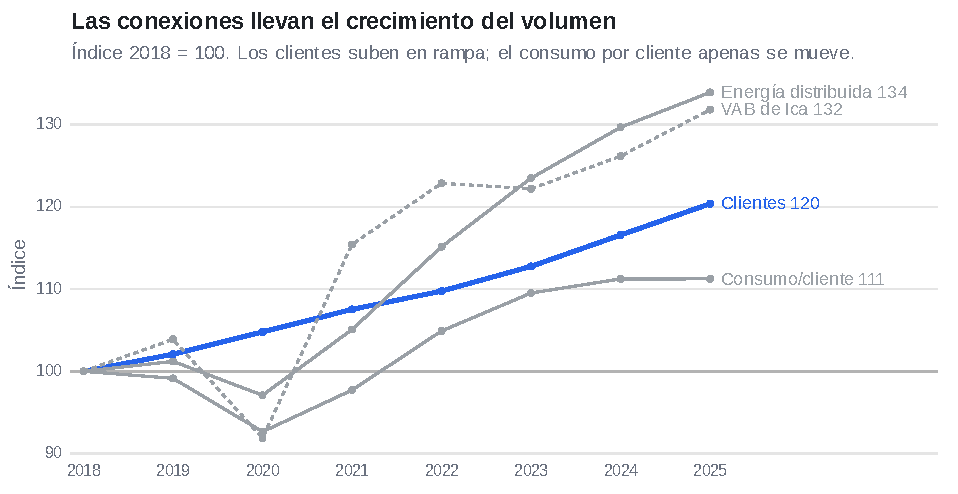
\includegraphics[width=\linewidth]{fig1_descomposicion.pdf}
\caption{Descomposición del crecimiento del volumen, índice 2018 = 100.
Elaboración propia sobre Memorias Anuales de ELDU e INEI.}
\label{fig:descomposicion}
\end{figure}

El VAB de Ica es la serie volátil: cae $12{.}3$\,\% en 2020 y rebota
$22{.}8$\,\% en 2021. El consumo por cliente acompaña ese ciclo con amplitud
mucho menor, y los clientes lo ignoran casi por completo: su serie es una rampa
de pendiente estable.

\begin{table}[H]
\centering
\caption{Tasas de crecimiento anual compuesto, 2018--2025.}
\small

\begin{tabular}{lr}
\toprule
Componente & CAGR (\%)\\
\midrule
Clientes & 2.65\\
Consumo por cliente & 1.52\\
Energía distribuida & 4.17\\
VAB real de Ica (driver) & 3.94\\
\bottomrule
\end{tabular}

\label{tab:descomposicion}
\end{table}

Las dos primeras filas del cuadro~\ref{tab:descomposicion} suman la tercera por
construcción. Las conexiones aportan el $64$\,\% del crecimiento del volumen, y
ese es el argumento para no estimar una elasticidad única sobre la energía
total: al hacerlo, el $2{.}65$\,\% de expansión de la base de clientes se le
atribuye al ingreso.

% ============================================================================
\section{Especificación}
% ============================================================================

El punto de partida es una identidad contable, no un supuesto:
\begin{equation}
Q_t = C_t\,q_t,
\qquad
\Delta \ln Q_t = \Delta \ln C_t + \Delta \ln q_t,
\end{equation}
donde $Q$ es la energía distribuida, $C$ el número de clientes y $q$ el consumo
por cliente. Los dos componentes responden a cosas distintas: las conexiones a
política de expansión de la concesionaria y a demografía, el consumo por
conexión al ingreso del hogar o del negocio conectado. La elasticidad-ingreso se
estima entonces sobre el segundo término.

Se estiman tres especificaciones del mismo parámetro, sobre el consumo por
cliente y, como contraste, sobre la energía total:
\begin{align}
\ln q_t &= \alpha + \eta \ln Y_t + \delta t + \varepsilon_t, \\
\ln q_t &= \alpha + \eta \ln Y_t + \varepsilon_t, \\
\Delta \ln q_t &= c + \eta\, \Delta \ln Y_t + u_t,
\end{align}
con $Y$ el VAB real de Ica. Los errores estándar son HAC (Newey--West), con
ancho de banda automático.

La especificación \textbf{en diferencias es la que se reporta como principal}, y
las de niveles quedan como corroboración. La razón es la muestra: con ocho
observaciones y series crecientes, $\ln Y$ y la tendencia determinista son casi
la misma variable, y separar el efecto ingreso del efecto tendencia se vuelve
frágil. La correlación entre ambas es $0{.}873$ y el factor de inflación de
varianza $4{.}2$ ---tolerable---, pero el estadístico de Durbin--Watson del
modelo en niveles ($1{.}13$, $p = 0{.}032$) rechaza la ausencia de
autocorrelación, lo que refuerza trabajar en diferencias.

La constante $c$ de la ecuación en diferencias tiene contenido propio: es el
crecimiento \emph{autónomo} del volumen, lo que la demanda crece con ingreso
plano. En la energía total resulta $2{.}93$\,\% anual, cifra del mismo orden que
el crecimiento observado de conexiones. Es la pieza que una regla de proyección
del tipo $Q(1+\eta g)$ descarta implícitamente al fijar la constante en cero.

La escalera de métodos se ajusta al $n$ disponible: las pruebas de raíz unitaria
(ADF), la de cointegración de Engle--Granger, el modelo de corrección de errores
y la validación fuera de muestra \textbf{se omiten}, por requerir 12 y 15
observaciones respectivamente. No se fuerzan sobre una muestra que no los
sostiene.

% ============================================================================
\section{Resultados}
% ============================================================================

\begin{table}[H]
\centering
\caption{Elasticidad-ingreso estimada por especificación. Errores estándar HAC
(Newey--West).}
\footnotesize

\begin{tabular}{lllrrcrrr}
\toprule
Bloque & Método & Rol & $\eta$ & EE & IC 95\% & $p$ & $n$ & $R^2$\\
\midrule
Por cliente & diferencias & \textbf{principal} & 0.320 & 0.082 & {}[0.110, 0.529] & 0.011 & 7 & 0.508\\
Por cliente & niveles & corrob. & 0.475 & 0.061 & {}[0.327, 0.624] & $<$0.001 & 8 & 0.800\\
Por cliente & niveles + tend. & corrob. & 0.411 & 0.139 & {}[0.053, 0.770] & 0.032 & 8 & 0.805\\
Energía total & diferencias & compar. & 0.315 & 0.085 & {}[0.096, 0.535] & 0.014 & 7 & 0.510\\
Energía total & niveles & compar. & 0.912 & 0.154 & {}[0.536, 1.288] & 0.001 & 8 & 0.854\\
Energía total & niveles + tend. & compar. & 0.400 & 0.164 & {}[-0.023, 0.823] & 0.059 & 8 & 0.938\\
Driver nacional & diferencias & robustez & 0.437 & 0.094 & {}[0.196, 0.677] & 0.006 & 7 & 0.526\\
Sin 2020--2021 & diferencias & robustez & 0.204 & 0.101 & {}[-0.117, 0.525] & 0.137 & 5 & 0.232\\
Volumen alternativo & diferencias & robustez & 0.309 & 0.043 & {}[0.199, 0.419] & 0.001 & 7 & 0.824\\
\bottomrule
\end{tabular}

\label{tab:estimaciones}
\end{table}

\begin{figure}[H]
\centering
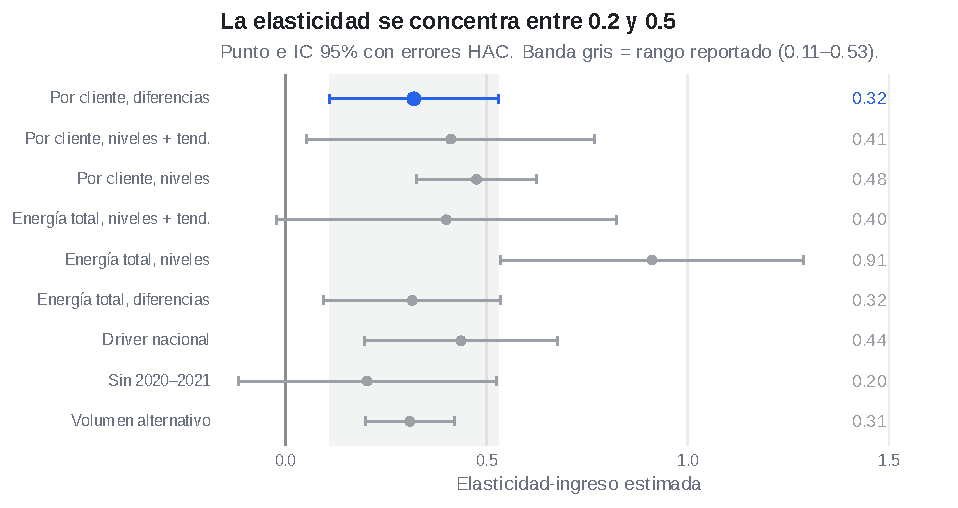
\includegraphics[width=\linewidth]{fig2_elasticidades.pdf}
\caption{Punto e intervalo de confianza al 95\,\% por especificación. La banda
gris marca el rango reportado.}
\label{fig:elasticidades}
\end{figure}

La especificación principal ---consumo por cliente, en diferencias--- da
$\eta = 0{.}320$, con error estándar HAC de $0{.}082$, $p = 0{.}011$ y
$R^2 = 0{.}508$ sobre siete diferencias. Las dos especificaciones en niveles
sobre la misma variable dan $0{.}411$ y $0{.}475$, de modo que las tres
convergen en una banda estrecha pese a apoyarse en supuestos distintos.

La fila que se despega es la de energía total en niveles y sin tendencia:
$0{.}912$. Es precisamente la que mezcla los dos procesos sin ningún término que
absorba el crecimiento de conexiones, de modo que atribuye al ingreso la rampa
de clientes. Que esa sea la única estimación cercana a la unidad es, en sí,
evidencia a favor de la descomposición.

\paragraph{Por qué un rango y no un punto.}
El intervalo de muestreo de la especificación principal mide $0{.}42$ de ancho,
por debajo del umbral que haría descartar un punto. Lo que fuerza el rango es
otra cosa: el estimador varía $0{.}156$ entre especificaciones igualmente
defendibles, por encima del umbral de $0{.}15$ fijado para esa prueba. Con ocho
observaciones, elegir entre niveles y diferencias mueve el resultado tanto como
el error de muestreo, y reportar un punto escondería esa segunda fuente de
incertidumbre.

% ============================================================================
\section{Diagnósticos y robustez}
% ============================================================================

\begin{table}[H]
\centering
\caption{Diagnósticos de los modelos sobre consumo por cliente. DW = Durbin--Watson, BG = Breusch--Godfrey de primer orden.}
\small

\begin{tabular}{lrrrrrrr}
\toprule
Modelo & $R^2$ & $R^2$ aj. & g.l. & DW & $p_{\text{DW}}$ & BG & $p_{\text{BG}}$\\
\midrule
Niveles (con tendencia) & 0.805 & 0.726 & 5 & 1.128 & 0.032 & 1.043 & 0.307\\
Diferencias & 0.508 & 0.409 & 5 & 1.107 & 0.140 & 1.151 & 0.283\\
\bottomrule
\end{tabular}

\label{tab:diagnosticos}
\end{table}

El modelo en niveles rechaza la ausencia de autocorrelación al 5\,\% según
Durbin--Watson; el de diferencias no. Breusch--Godfrey de primer orden no
rechaza en ninguno, aunque con cinco grados de libertad su potencia es baja.

\paragraph{Estabilidad.}
Excluyendo una observación a la vez, el estimador se mueve en el rango
$[0{.}146,\;0{.}532]$. La observación más influyente es 2021, cuyo retiro
desplaza el parámetro $0{.}212$. Con ocho datos, una sola observación mueve el
resultado tanto como el intervalo de confianza completo.

\paragraph{Robustez.}
Los tres chequeos, todos sobre la especificación en diferencias, están en las
últimas filas del cuadro~\ref{tab:estimaciones}. El más informativo y el más
incómodo es el tercero. El desplome de 2020 y el rebote de 2021 aportan buena
parte de la variación que identifica el parámetro: el VAB de Ica cayó
$12{.}3$\,\% y rebotó $22{.}8$\,\%, contra $4{.}2$\,\% y $7{.}9$\,\% en la
energía. Retirados esos dos años quedan cinco diferencias, el punto estimado
baja a $0{.}204$ y el intervalo cruza el cero ($p = 0{.}137$). El signo se
mantiene, pero la precisión depende del episodio pandemia.

La lectura razonable es que la elasticidad está acotada por arriba con holgura
---todas las especificaciones y chequeos quedan por debajo de $0{.}7$, excepto
la de niveles sin tendencia sobre energía total, que es la sesgada--- y que su
límite inferior no es distinguible de cero con esta muestra.

% ============================================================================
\section{Proyección}
% ============================================================================

La descomposición obliga a una regla de proyección con dos términos, uno por
cada proceso:
\begin{equation}
Q_{t+1} = Q_t\,\bigl(1 + g^{C}_{t+1}\bigr)\bigl(1 + \eta\, g^{Y}_{t+1}\bigr).
\label{eq:proyeccion}
\end{equation}

\begin{figure}[H]
\centering
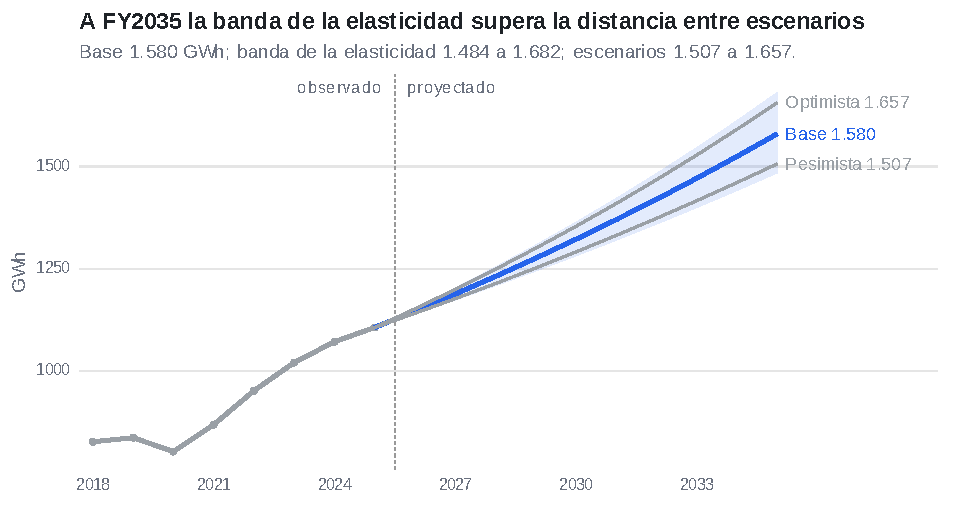
\includegraphics[width=\linewidth]{fig3_proyeccion.pdf}
\caption{Volumen observado y proyectado a FY2035. La banda recoge únicamente la
incertidumbre de $\eta$.}
\label{fig:proyeccion}
\end{figure}

\begin{table}[H]
\centering
\caption{Volumen proyectado a FY2035 por escenario.}
\small

\begin{tabular}{lrrrr}
\toprule
Escenario & $g$ ingreso & GWh central & GWh banda inf. & GWh banda sup.\\
\midrule
Base & 3.0\% & 1 580 & 1 484 & 1 682\\
Optimista & 4.5\% & 1 657 & 1 509 & 1 818\\
Pesimista & 1.5\% & 1 507 & 1 460 & 1 555\\
\bottomrule
\end{tabular}

\label{tab:proyeccionfin}
\end{table}

Los tres escenarios se distinguen únicamente por el crecimiento supuesto del
ingreso ($3{.}0$\,\%, $4{.}5$\,\% y $1{.}5$\,\% anual). Que la banda sea más
ancha que la separación entre escenarios dice algo útil: con esta muestra, el
error de estimación del parámetro pesa más sobre el volumen a diez años que la
diferencia entre un escenario macroeconómico bueno y uno malo.

\paragraph{El supuesto que manda es el otro.}
El crecimiento de conexiones se fija en $2{.}65$\,\% anual, el CAGR observado,
sostenido hasta 2035. No es una estimación: es un supuesto, y mueve el resultado
más que $\eta$, porque entra sin atenuar mientras $\eta$ multiplica un
crecimiento del ingreso de $3$\,\%. Una convergencia gradual a una tasa menor
---lo esperable conforme la cobertura se satura--- bajaría la proyección de
forma apreciable.

Un contraste útil para calibrar: aplicar la elasticidad estimada dentro de una
regla de un solo término, $Q(1+\eta g)$, da $0{.}96$\,\% anual, muy por debajo
del $4{.}17$\,\% observado en el periodo muestral. No es que $\eta$ sea baja: es
que esa regla no tiene dónde poner las conexiones. El detalle anual de la
proyección está en el apéndice~\ref{ap:proyeccion}.

% ============================================================================
\section{Limitaciones}
% ============================================================================

\begin{enumerate}
  \item \textbf{Ocho observaciones.} Es la restricción que manda y la que define
  qué se pudo hacer. Quedan fuera las pruebas de raíz unitaria, la
  cointegración, el modelo de corrección de errores y la validación fuera de
  muestra. Los intervalos son anchos por construcción.
  \item \textbf{Los intervalos son además optimistas.} Los errores HAC son
  asintóticos: con $n$ de un dígito su cobertura real queda por debajo del
  95\,\% nominal. El intervalo reportado subestima la incertidumbre, y es otra
  razón para leer $\eta$ como rango.
  \item \textbf{Frecuencia anual.} El registro mensual de Osinergmin (SICOM)
  requiere solicitud formal y no se usó. Toda la dinámica intra-anual
  ---estacionalidad del agro de Ica, efectos tarifarios, rezagos de ajuste---
  queda invisible. Con datos mensuales la muestra permitiría un ARDL o un ECM
  completo.
  \item \textbf{El choque de 2020--2021 pesa demasiado.} Retirar esos dos años
  lleva el parámetro de $0{.}32$ a $0{.}20$ y vuelve el intervalo no
  significativo.
  \item \textbf{Sin desagregado por tensión.} Las ventas por segmento arrancan
  en 2022. No es posible estimar elasticidades separadas de baja y media
  tensión, ni para clientes libres.
  \item \textbf{Conexiones no modeladas.} El crecimiento de clientes entra como
  proceso exógeno, no estimado. Dado que explica dos tercios del crecimiento del
  volumen, cualquier proyección depende más de ese supuesto que de $\eta$.
  Modelarlo exigiría datos de cobertura, vivienda y expansión de red que no
  están aquí.
  \item \textbf{El driver regional tiene su propio ruido.} El VAB de Ica está
  dominado por minería, manufactura y agroexportación, cuyo ciclo no coincide
  con el consumo eléctrico del padrón de ELDU: en 2023 el VAB cayó $0{.}5$\,\%
  mientras la energía creció $7{.}0$\,\%. Los últimos años son preliminares y
  estimados, y se revisan.
  \item \textbf{Precisión desigual de la dependiente.} Los años 2018--2021
  provienen de la lectura de un gráfico; 2022--2025, de cuadros.
\end{enumerate}

% ============================================================================
\section{Reproducibilidad}
% ============================================================================

Todo el trabajo corre con \texttt{Rscript run\_all.R} sobre R 4.3.3, con semilla
20261007. El repositorio está en la rama
\texttt{claude/wizardly-clarke-prjkt1} de \texttt{afmendezsuarez-a11y/Claude}.

La cadena va de la descarga a la estimación en scripts numerados: adquisición
(\texttt{01}--\texttt{04}), preparación de la serie anual (\texttt{04b}),
construcción del panel (\texttt{05}), estimación (\texttt{06}), proyección
(\texttt{07}), informe (\texttt{08}) y, para este documento, figuras
(\texttt{09}) y tablas (\texttt{10}). Ni las figuras ni las tablas de este PDF
se editan a mano: se generan desde las salidas del pipeline, de modo que el
documento compila lo que la corrida produjo.

Dos propiedades condicionan qué se puede creer de las cifras:

\begin{itemize}
  \item \textbf{Trazabilidad.} Cada archivo de entrada queda registrado en
  \texttt{data/raw/SOURCES.md} con su descripción, tamaño y hash SHA256. Toda
  cifra del documento se remonta a un archivo de \texttt{data/raw/}.
  \item \textbf{Sin datos sintetizados.} No existe ninguna ruta de datos
  simulados, de demostración o imputados en el repositorio. Si falta un insumo
  obligatorio, la construcción del panel se detiene con código de salida 2 y
  documenta qué falta, en vez de rellenar. La serie de energía pasa además una
  validación de plausibilidad ---rango de magnitud, mínimo de observaciones y
  tope de $60$\,\% al salto interanual--- que rechaza extracciones mal alineadas
  antes de estimar.
\end{itemize}

Las pruebas de integración (\texttt{tests/integration\_smoke.R}) corren el
pipeline completo en un directorio aislado sobre tres tamaños de muestra, con un
parámetro conocido, y verifican que el estimador lo recupere, que la
descomposición reconstruya el crecimiento de conexiones y que el método
reportado corresponda al $n$ disponible. La serie de prueba es artificial, vive
en un directorio temporal y el pipeline no tiene ninguna ruta que la use: es
prueba de código, no un modo de demostración.

\appendix

% ============================================================================
\section{Panel anual}\label{ap:panel}
% ============================================================================

\begin{table}[H]
\centering
\caption{Panel anual utilizado en la estimación.}
\small

\begin{tabular}{lrrrr}
\toprule
Año & Energía (GWh) & Clientes & MWh/cliente & VAB Ica (miles S/)\\
\midrule
2018 & 826 & 240 981 & 3.428 & 16 994 391\\
2019 & 836 & 245 990 & 3.399 & 17 656 354\\
2020 & 802 & 252 523 & 3.176 & 15 612 472\\
2021 & 868 & 259 125 & 3.350 & 19 614 370\\
2022 & 951 & 264 480 & 3.596 & 20 877 156\\
2023 & 1020 & 271 718 & 3.754 & 20 766 164\\
2024 & 1071 & 280 907 & 3.813 & 21 439 833\\
2025 & 1106 & 290 074 & 3.813 & 22 399 353\\
\bottomrule
\end{tabular}

\end{table}

% ============================================================================
\section{Proyección anual completa}\label{ap:proyeccion}
% ============================================================================

\begin{table}[H]
\centering
\caption{Volumen proyectado por escenario, GWh. La banda corresponde al
intervalo de $\eta$ aplicado al escenario base.}
\small

\begin{tabular}{lrrrrr}
\toprule
Año & Base & Optimista & Pesimista & Banda inf. & Banda sup.\\
\midrule
2026 & 1146 & 1152 & 1141 & 1139 & 1153\\
2027 & 1188 & 1199 & 1177 & 1173 & 1203\\
2028 & 1231 & 1249 & 1214 & 1208 & 1254\\
2029 & 1276 & 1300 & 1252 & 1244 & 1308\\
2030 & 1322 & 1354 & 1291 & 1281 & 1364\\
2031 & 1370 & 1410 & 1331 & 1320 & 1422\\
2032 & 1420 & 1468 & 1373 & 1359 & 1483\\
2033 & 1471 & 1528 & 1416 & 1400 & 1546\\
2034 & 1525 & 1591 & 1461 & 1441 & 1613\\
2035 & 1580 & 1657 & 1507 & 1484 & 1682\\
\bottomrule
\end{tabular}

\end{table}

\end{document}
